%%%%%%%%%%%%%%%%%%%%%%%%%%%%%%%%%%%%%
%                                   %
% Compile with XeLaTeX and biber    %
%                                   %
% Questions or comments:            %
%                                   %
% joshua dot mcneill at uga dot edu %
%                                   %
%%%%%%%%%%%%%%%%%%%%%%%%%%%%%%%%%%%%%

\documentclass{beamer}
  % Read in standard preamble (cosmetic stuff)
  %%%%%%%%%%%%%%%%%%%%%%%%%%%%%%%%%%%%%%%%%%%%%%%%%%%%%%%%%%%%%%%%
% This is a standard preamble used in for all slide documents. %
% It basically contains cosmetic settings.                     %
%                                                              %
% Joshua McNeill                                               %
% joshua dot mcneill at uga dot edu                            %
%%%%%%%%%%%%%%%%%%%%%%%%%%%%%%%%%%%%%%%%%%%%%%%%%%%%%%%%%%%%%%%%

% Beamer settings
% \usetheme{Berkeley}
\usetheme{CambridgeUS}
% \usecolortheme{dove}
% \usecolortheme{rose}
\usecolortheme{seagull}
\usefonttheme{professionalfonts}
\usefonttheme{serif}
\setbeamertemplate{bibliography item}{}

% Packages and settings
\usepackage{fontspec}
  \setmainfont{Charis SIL}
\usepackage{hyperref}
  \hypersetup{colorlinks=true,
              allcolors=blue}
\usepackage{graphicx}
  \graphicspath{{../../figures/}}
\usepackage[normalem]{ulem}
\usepackage{enumerate}

% Document information
\author{M. McNeill}
\title[FREN2001]{Français 2001}
\institute{\url{joshua.mcneill@uga.edu}}
\date{}

%% Custom commands
% Lexical items
\newcommand{\lexi}[1]{\textit{#1}}
% Gloss
\newcommand{\gloss}[1]{`#1'}
\newcommand{\tinygloss}[1]{{\tiny`#1'}}
% Orthographic representations
\newcommand{\orth}[1]{$\langle$#1$\rangle$}
% Utterances (pragmatics)
\newcommand{\uttr}[1]{`#1'}
% Sentences (pragmatics)
\newcommand{\sent}[1]{\textit{#1}}
% Base dir for definitions
\newcommand{\defs}{../definitions}


  % Packages and settings

  % Document information
  \subtitle[Indéfinies et négatives]{Les expressions indéfinies et négatives}

\begin{document}
  % Read in the standard intro slides (title page and table of contents)
  \begin{frame}
    \titlepage
    \tiny{Office: % Basically a variable for office hours location
Gilbert 121\\
          Office hours: % Basically a variable for office hours
 lundi, mercredi, vendredi 10:10--11:10
}
  \end{frame}

  \begin{frame}{Quelque chose ou rien}
    \scriptsize
    \begin{columns}
      \column{0.5\textwidth}
        \begin{enumerate}
          \item On a vu \alert{quelque chose} sur la table?
          \item<2->[$\to$] Non, on n'a \alert{rien} vu sur la table.
          \item<3-> \alert{Quelqu'un} lui téléphone?
          \item<4->[$\to$] Non, \alert{personne ne} lui téléphone.
          \item<5-> Il n'y a \alert{personne} à la porte?
          \item<6->[$\to$] Si, il y a \alert{quelqu'un} à la porte.
          \item<7-> Tu vas manger au Grit \alert{quelquefois}?
          \item<8->[$\to$] Non, je ne vais \alert{jamais} manger au Grit.
          \item<9-> Il va donner \textcolor{red}{quelque chose} à \textcolor{purple}{quelqu'un}?
          \item<10->[$\to$] Non, il ne va \textcolor{red}{rien} donner à \textcolor{purple}{personne}.
        \end{enumerate}
      \column{0.5\textwidth}
        \begin{minipage}[c][0.8\textheight]{\linewidth}
          \begin{center}
            \only<1-2>{
              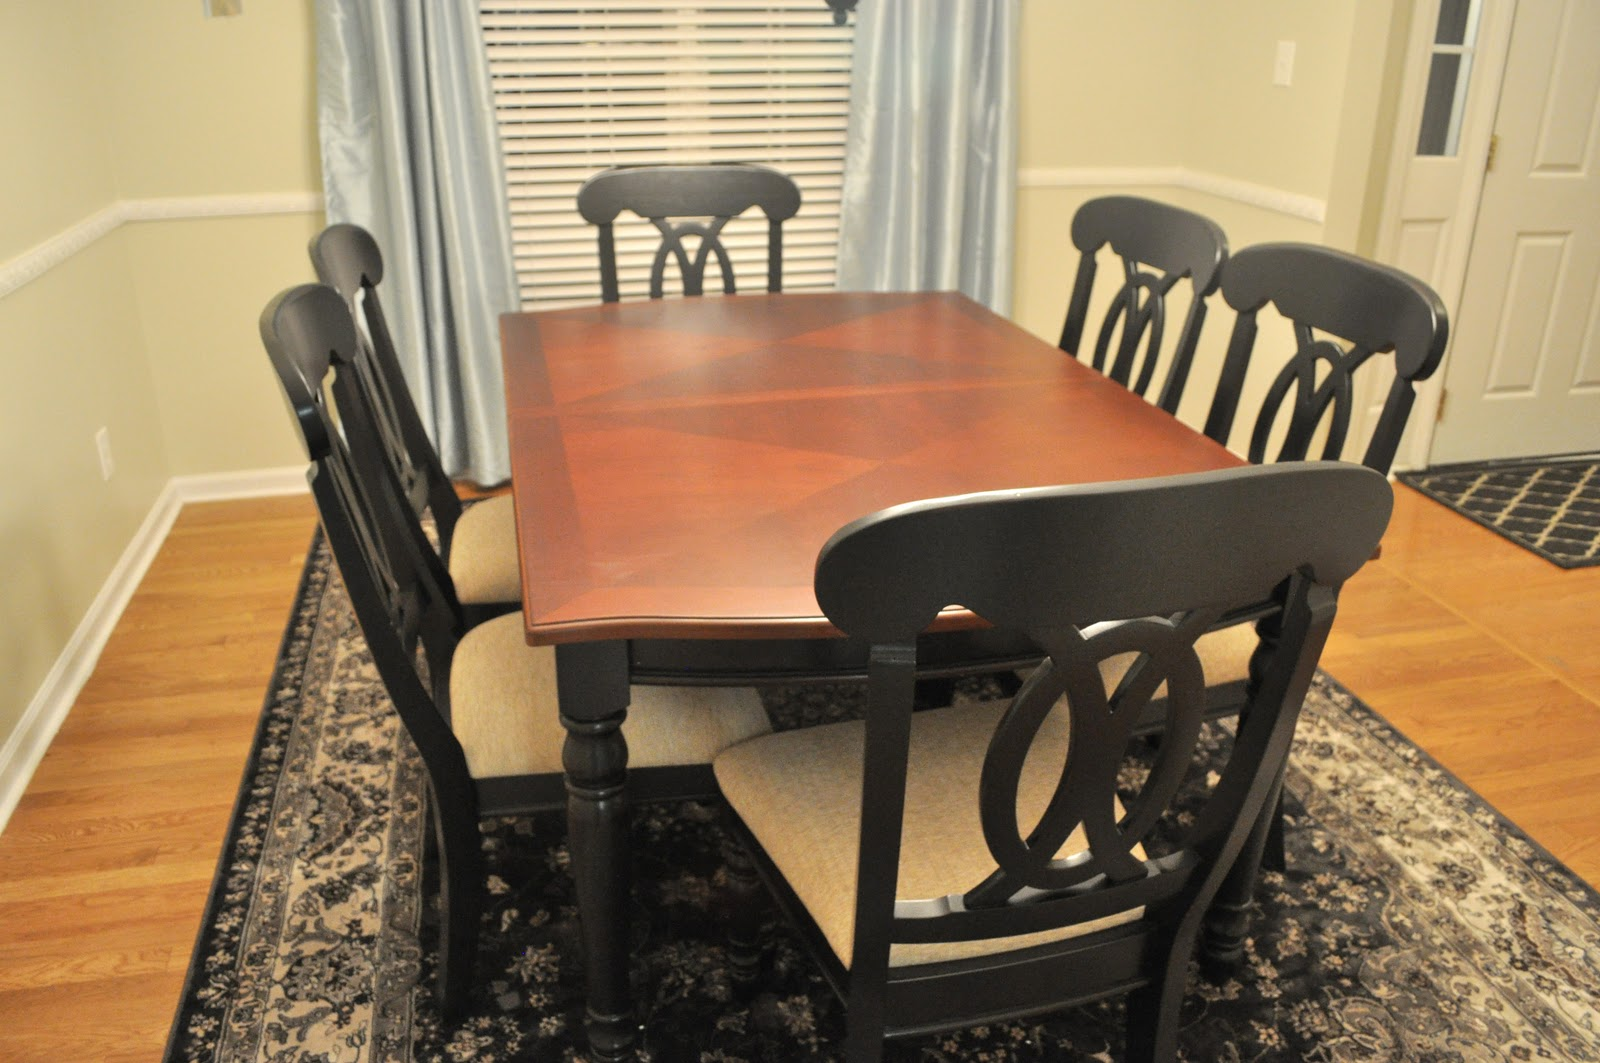
\includegraphics[scale=0.105]{table.jpg}
            }
            \only<3-4>{
              
\includegraphics[scale=0.14]{téléphone.jpg}
            }
            \only<5-6>{
              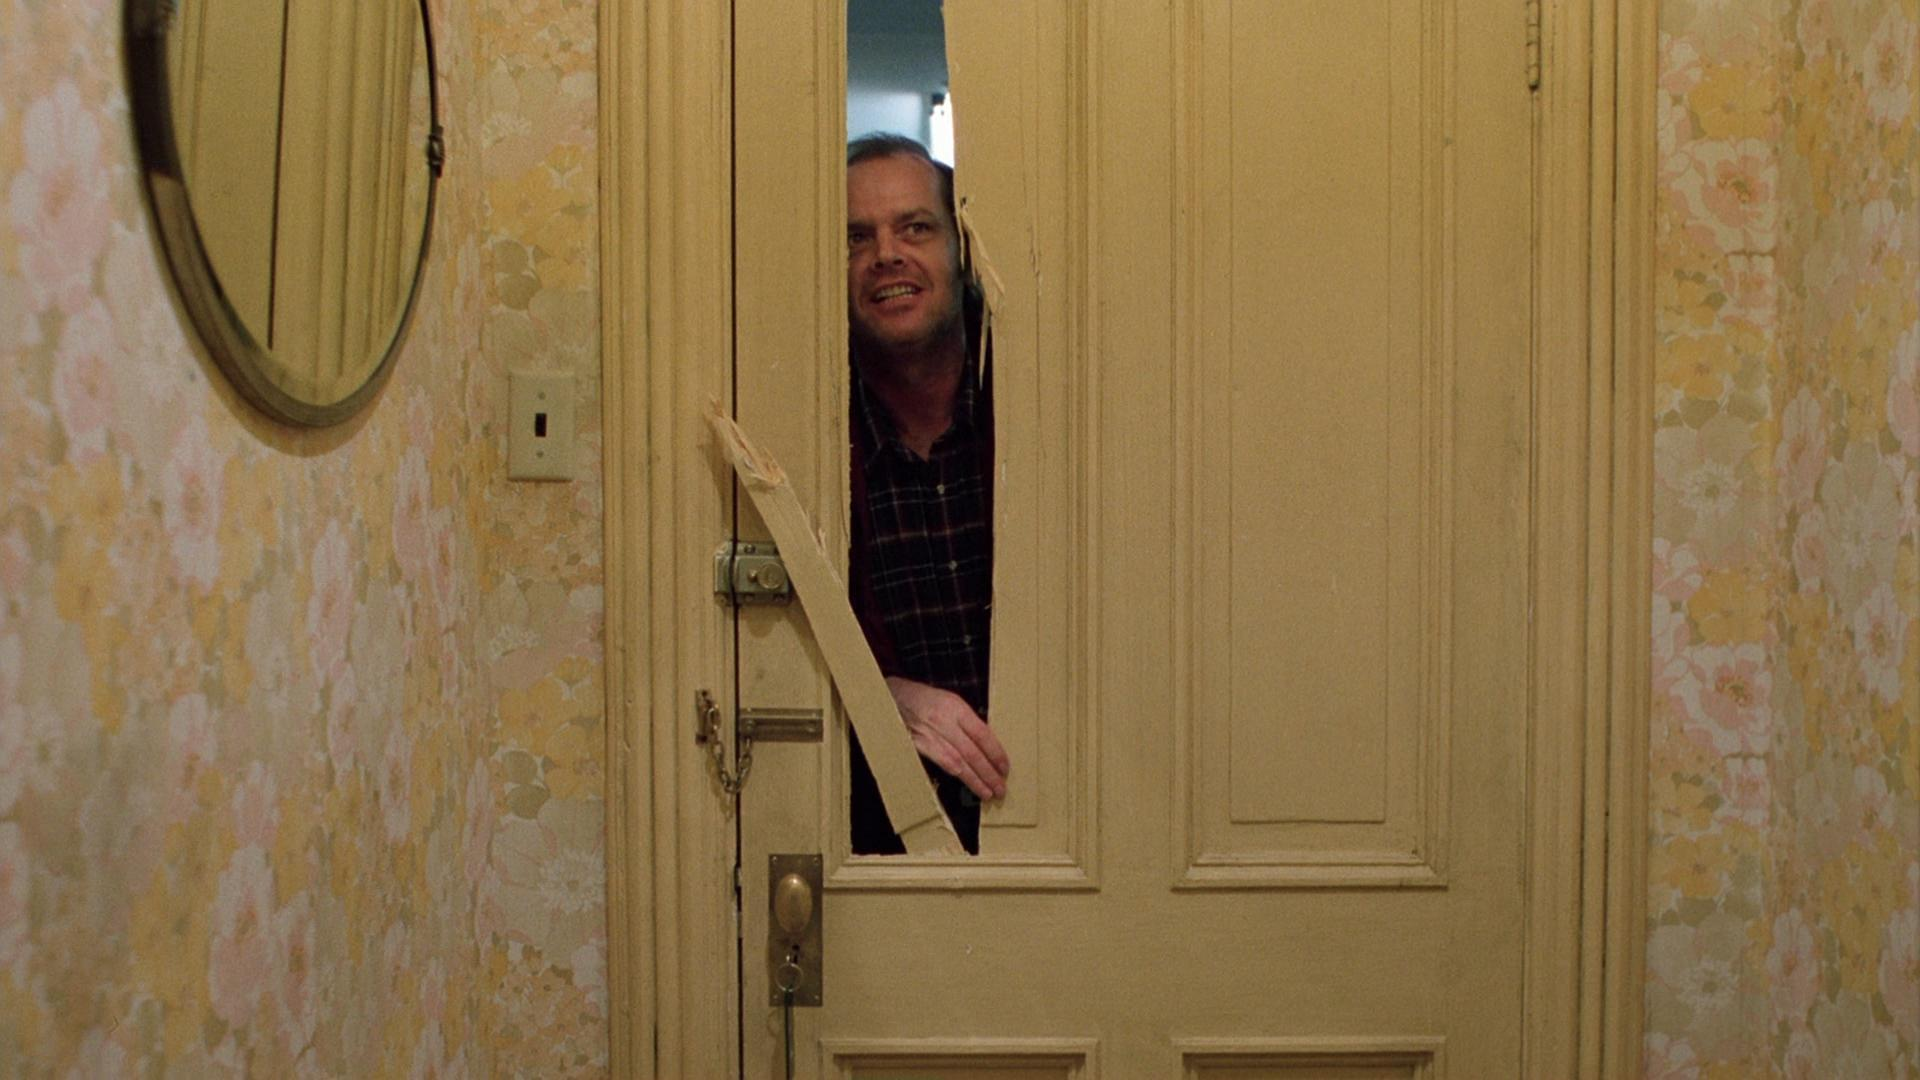
\includegraphics[scale=0.12]{porte.jpg}
            }
            \only<7-8>{
              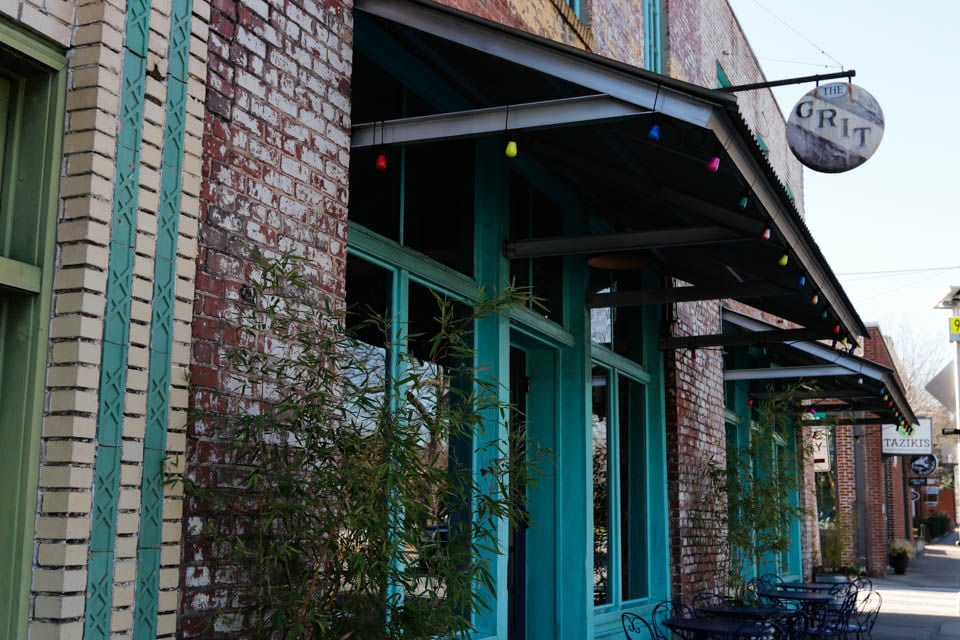
\includegraphics[scale=0.17]{grit.jpg}
            }
            \only<9-10>{
              
\includegraphics[scale=0.125]{bezos.jpg}
            }
          \end{center}
        \end{minipage}
    \end{columns}
  \end{frame}

  \begin{frame}{}
    \begin{center}
      \Large Quiz
    \end{center}
  \end{frame}

  \begin{frame}{Quand ça arrive}
    \scriptsize
    Avec un/e partenaire, discutez de ce qui se passe \gloss{what happens} quand vous êtes dans les situations suivantes.
    Utilisez les expressions indéfinies (\lexi{quelquefois}, \lexi{quelque chose}, \lexi{quelqu'un}) et négatives (\lexi{ne...jamais}, \lexi{ne...rien}, \lexi{ne...personne}).
    \begin{description}
      \item[] \textbf{Modèle:} \emph{quand vous allez au supermarché}
      \item[E1:] J'achète \alert{quelquefois} des légumes, mais je n'achète \alert{jamais} de viande. Et toi?
      \item[E2:] Moi, je n'y vas avec \alert{personne}, parce que je ne vais pas au supermarché.
      \item[E1:] Mais, comment est-ce tu manges?
    \end{description}
    \vspace{0.3cm}
    Qu'est ce qui se passe ...
    \begin{columns}[t]
      \column{0.5\textwidth}
        \begin{enumerate}
          \item quand vous passez des fêtes en famille?
          \item quand vous sortez avec des amis le week-end?
          \item quand vous partez en vacances en famille?
        \end{enumerate}
      \column{0.5\textwidth}
        \begin{enumerate}
          \setcounter{enumi}{3}
          \item quand vous avez beaucoup de travail à la fac?
          \item quand vous n'avez pas beaucoup d'argent?
          \item quand vous vous disputez avec des amis?
        \end{enumerate}
    \end{columns}
  \end{frame}

  \begin{frame}{}
    \begin{center}
      \Large Questions?
    \end{center}
  \end{frame}
\end{document}
